\chapter{Méthodologie et Cycle de Vie}

\section{Choix de la Méthodologie}

Face à un projet comportant une forte \textbf{incertitude technique} (technologies nouvelles, architecture distribuée), nous avons opté pour une approche \textbf{Agile (Scrum + Kanban)}, conformément au Chapitre 4 du cours (Cycles de vie).

\begin{table}[H]
\centering
\begin{tabularx}{\textwidth}{L{3.5cm} C{3cm} C{3cm} C{3cm}}
\toprule
\textbf{\color{primarycolor}Critère} &
\textbf{\color{primarycolor}Cascade} &
\textbf{\color{primarycolor}Agile (Scrum)} &
\textbf{\color{primarycolor}Notre choix} \\
\midrule
Besoins évolutifs & Figés au début & Adaptatifs & \textbf{Agile} \\
\addlinespace[0.1cm]
Livraison & Unique à la fin & Incrémentale & \textbf{Agile} \\
\addlinespace[0.1cm]
Feedback & Tardif & Continu & \textbf{Agile} \\
\addlinespace[0.1cm]
Risques & Détectés tard & Détectés tôt & \textbf{Agile} \\
\addlinespace[0.1cm]
Documentation & Lourde & Légère et utile & \textbf{Agile} \\
\bottomrule
\end{tabularx}
\caption{Comparaison Cascade vs Agile pour notre projet}
\end{table}

Notre projet est un \textbf{projet d'innovation} avec des technologies nouvelles (Kafka, Flink). L'approche Agile nous a permis d'avancer par itérations courtes et de valider progressivement.

\section{Approche Agile (Scrum)}

Plutôt que de livrer tout à la fin, nous avons procédé par \textbf{itérations courtes} (Sprints de 3 à 5 jours). À la fin de chaque Sprint, une phase de \textbf{validation (Recette)} a permis à la MOA de vérifier les livrables :

\begin{enumerate}
    \item \textbf{Sprint 1} : Conteneurs Docker opérationnels et topic Kafka fonctionnel~;
    \item \textbf{Sprint 2} : Simulateur et topologies traitent correctement les données~;
    \item \textbf{Sprint 3} : Le replay produit des résultats cohérents.
\end{enumerate}

\section{Utilisation de Taiga (Kanban)}

Pour gérer le flux de travail au quotidien, nous avons mis en place un \textbf{tableau Kanban} sur \textbf{Taiga}, organisé en 5 colonnes : \textit{New}, \textit{Ready}, \textit{In Progress}, \textit{Ready for Test} et \textit{Done}.

\begin{borderedfigure}
    \centering
    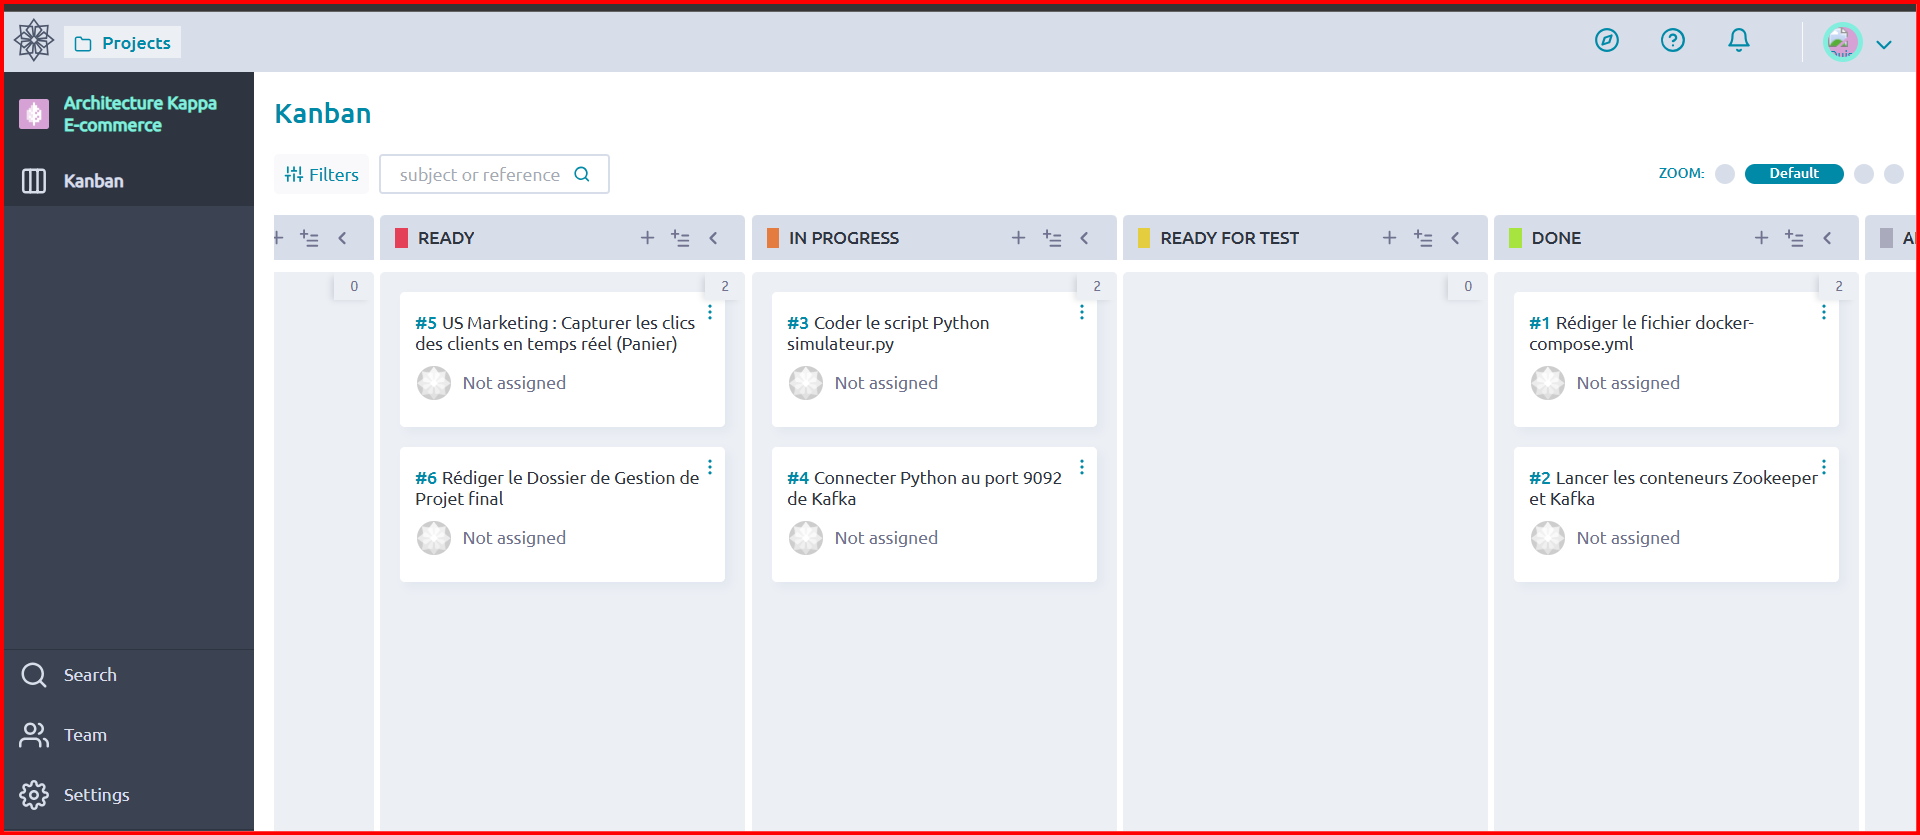
\includegraphics[width=\textwidth]{../screenshots/taiga.png}
    \captionof{figure}{Tableau Kanban du projet sur Taiga}
\end{borderedfigure}

Cet outil nous a permis de visualiser les User Stories, suivre leur état d'avancement et identifier les goulots d'étranglement dans le processus.

\section{Outils Agile Utilisés}

\begin{table}[H]
\centering
\begin{tabularx}{\textwidth}{L{3.5cm} X L{4cm}}
\toprule
\textbf{\color{primarycolor}Outil} &
\textbf{\color{primarycolor}Rôle} &
\textbf{\color{primarycolor}Référence cours} \\
\midrule
\textbf{Taiga} & Kanban board, suivi des User Stories & Ch.5 --- Suivi du projet \\
\addlinespace[0.1cm]
\textbf{GanttProject} & Planification temporelle, chemin critique & Ch.7 --- Planification \\
\addlinespace[0.1cm]
\textbf{Git} & Versioning du code source & Bonne pratique DevOps \\
\addlinespace[0.1cm]
\textbf{Docker} & Déploiement reproductible & Sprint 1 \\
\bottomrule
\end{tabularx}
\caption{Outils Agile et leur correspondance avec le cours}
\end{table}
